% generated by scripts/pkl_to_latex.py
% source PKL : nscan_v1_L8_U10_t1_mode-uniform_nmin2_solver-gcg_full_restarts10_iter300_kmax2_tol1em09_N3to8_n6-d2c9afae4595.pkl
% scan type  : nscan
% state      : gs
% quantity   : vn-entropy
% requires   : \usepackage{pgfplots} \pgfplotsset{compat=1.18}
% colours match the matplotlib PDF (tab10 cycle)
\definecolor{gmeC0}{HTML}{1F77B4}
\definecolor{gmeC1}{HTML}{FF7F0E}
\definecolor{gmeC2}{HTML}{2CA02C}
\definecolor{gmeC3}{HTML}{D62728}
\definecolor{gmeC4}{HTML}{9467BD}
\definecolor{gmeC5}{HTML}{8C564B}
\definecolor{gmeC6}{HTML}{E377C2}
\definecolor{gmeC7}{HTML}{17BECF}

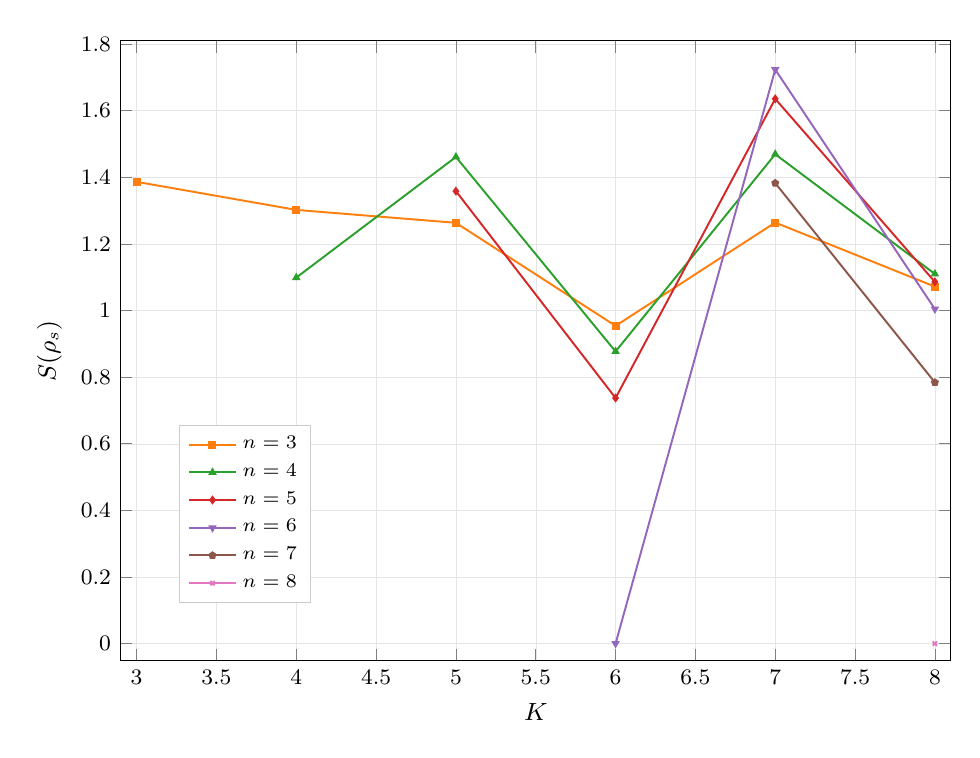
\begin{tikzpicture}
  \begin{axis}[
    width=\columnwidth,
    height=0.78\columnwidth,
    xlabel={$K$},
    ylabel={$S(\rho_s)$},
    grid=both,
    grid style={line width=.1pt, draw=gray!20},
    tick label style={font=\footnotesize\rmfamily, /pgf/number format/fixed},
    label style={font=\small\rmfamily},
    scaled ticks=false,
    legend style={font=\scriptsize\rmfamily, draw=gray!40, at={(0.5,1.03)}, anchor=south, /tikz/every even column/.append style={column sep=6pt}},
    legend cell align={left},
    legend columns=1,
    ymin=-0.052,
    ymax=1.81,
    xmin=2.9,
    xmax=8.1,
    legend style={at={(0.150,0.237)}, anchor=center, fill=white},
  ]
    \addplot[color=gmeC1, mark=square*, mark size=1.1pt, line width=0.7pt] coordinates {
        (3,1.386294) (4,1.301956) (5,1.263182) (6,0.953743)
        (7,1.264035) (8,1.071622)
    };
    \addlegendentry{$n=3$}
    \addplot[color=gmeC2, mark=triangle*, mark size=1.1pt, line width=0.7pt] coordinates {
        (4,1.098612) (5,1.460915) (6,0.876873) (7,1.469137)
        (8,1.109563)
    };
    \addlegendentry{$n=4$}
    \addplot[color=gmeC3, mark=diamond*, mark size=1.1pt, line width=0.7pt] coordinates {
        (5,1.358282) (6,0.737197) (7,1.635406) (8,1.085902)
    };
    \addlegendentry{$n=5$}
    \addplot[color=gmeC4, mark=triangle*, mark size=1.1pt, mark options={rotate=180}, line width=0.7pt] coordinates {
        (6,0) (7,1.723473) (8,1.004235)
    };
    \addlegendentry{$n=6$}
    \addplot[color=gmeC5, mark=pentagon*, mark size=1.1pt, line width=0.7pt] coordinates {
        (7,1.382389) (8,0.783959)
    };
    \addlegendentry{$n=7$}
    \addplot[color=gmeC6, mark=x, mark size=1.1pt, line width=0.7pt] coordinates {
        (8,0)
    };
    \addlegendentry{$n=8$}
  \end{axis}
\end{tikzpicture}
